\documentclass[11pt,a4paper]{article}

% Configuración de página y márgenes
\usepackage[margin=1in, top=1.2in, bottom=1.2in]{geometry}

% Paquetes para caracteres especiales y codificación
\usepackage[utf8]{inputenc}
\usepackage[T1]{fontenc}
\usepackage{lmodern}
\usepackage{textcomp}
\usepackage{amsmath}
\usepackage{amssymb}
\usepackage{gensymb}

% Soporte para idiomas (español e inglés)
\usepackage[spanish,english]{babel}

% Paquetes para imágenes y gráficos
\usepackage{graphicx}
\usepackage{float}
\usepackage{caption}
\usepackage{subcaption}

% Paquetes para tablas
\usepackage{longtable}
\usepackage{booktabs}
\usepackage{array}
\usepackage{multirow}
\usepackage{multicol}
\usepackage{tabularx}

% Control de saltos de página
\usepackage{needspace}
\usepackage{afterpage}
\usepackage{placeins}

% Enlaces e hipervínculos
\usepackage[colorlinks=true, linkcolor=blue, urlcolor=blue, citecolor=blue]{hyperref}

% Paquetes para código y verbatim
\usepackage{fancyvrb}
\usepackage{listings}
\usepackage{xcolor}

% Paquetes para diseño profesional
\usepackage{tcolorbox}
\usepackage{tikz}
\tcbuselibrary{most}
\usepackage{fancyhdr}
\usepackage{lastpage}

% Configuración de encabezados y pies de página
\pagestyle{fancy}
\fancyhf{} % Limpiar encabezados y pies

% Pie de página
\fancyfoot[L]{\small UNIT Electronics - Development}
\fancyfoot[C]{\small 2025-07-21}
\fancyfoot[R]{\small Page \thepage\ of \pageref{LastPage}}

% Línea en encabezado y pie
\renewcommand{\headrulewidth}{0.4pt}
\renewcommand{\footrulewidth}{0.4pt}

% Estilo para primera página de cada sección
\fancypagestyle{plain}{
    \fancyhf{}
    \fancyfoot[L]{\small UNIT Electronics - Development}
    \fancyfoot[C]{\small 2025-07-21}
    \fancyfoot[R]{\small Page \thepage\ of \pageref{LastPage}}
    \renewcommand{\headrulewidth}{0pt}
    \renewcommand{\footrulewidth}{0.4pt}
}

% Configuración de listings para código
\lstset{
    basicstyle=\ttfamily\small,
    breaklines=true,
    frame=single,
    backgroundcolor=\color{gray!10},
    keywordstyle=\color{blue},
    commentstyle=\color{green!50!black},
    stringstyle=\color{red}
}

% Paquetes para mejor tipografía
\usepackage{microtype}
\usepackage{setspace}

% Configuración de espaciado
\onehalfspacing

% Comandos personalizados
\providecommand{\tightlist}{}

% Comando para evitar viudas y huérfanas
\widowpenalty=10000
\clubpenalty=10000

% Configuración de profundidad de numeración
\setcounter{secnumdepth}{3}
\setcounter{tocdepth}{3}

\begin{document}


% Página de título estandarizada IEEE/ISO
\begin{titlepage}
    \centering
    
    % Header corporativo estandarizado
    \vspace*{0.5cm}
    
    % Logo y información corporativa
    \begin{minipage}{0.3\textwidth}
        \centering
        
        
\includegraphics[width=\textwidth]{logo.png}
        
    \end{minipage}
    \hfill
    \begin{minipage}{0.6\textwidth}
        \raggedleft
        {\small \textbf{UNIT Electronics}}\\
        {\footnotesize Technical Documentation}\\
        {\footnotesize Development Project - Prototype Phase}
    \end{minipage}
    
    \vspace{0.5cm}
    
    % Línea divisoria principal
    {\color{blue}\rule{\textwidth}{2pt}}
    
    \vspace{1.5cm}
    
    % Clasificación del documento
    \begin{tcolorbox}[
        colback=blue!5!white,
        colframe=blue!75!black,
        width=0.9\textwidth,
        arc=2mm,
        boxrule=1.5pt,
        halign=center
    ]
    {\Large \textbf{TECHNICAL DATASHEET}}\\[0.2cm]
    {\normalsize Hardware Documentation \& Development Specifications}
    \end{tcolorbox}
    
    \vspace{0.8cm}
    
    % Título principal estandarizado
    {\Huge \textbf{\textcolor{blue}{ICP-10111 Sensor de Presión Barométrica}}}\\[0.3cm]
    
    % Subtítulo técnico
    
    {\LARGE \textcolor{gray}{Módulo Sensor Ambiental de Alta Precisión}}\\[0.5cm]
    
    
    % Código de parte y versión
    \begin{tcolorbox}[
        colback=gray!10!white,
        colframe=gray!50!black,
        width=0.7\textwidth,
        arc=1mm,
        boxrule=1pt
    ]
    \centering
    \begin{tabular}{l l}
    \textbf{Part Number:} & ICP-10111-001 \\
    \textbf{Revision:} & Rev. 1.0 \\
    \textbf{Document Date:} & 2025-07-21
    \end{tabular}
    \end{tcolorbox}
    
    \vspace{1cm}
    
    % Tabla de información del documento (Formato simplificado)
    \begin{tcolorbox}[
        colback=white,
        colframe=black,
        width=0.9\textwidth,
        arc=0mm,
        boxrule=1pt,
        halign=center
    ]
    {\normalsize \textbf{DOCUMENT INFORMATION}}\\[0.3cm]
    \begin{tabular}{|l|l|}
    \hline
    \textbf{Document Type} & Technical Datasheet \\
    \hline
    \textbf{Classification} & Documentación de Desarrollo \\
    \hline
    \textbf{Project Phase} & Prototype \& Development \\
    \hline
    
    \textbf{Technical Author} & Equipo de Ingeniería DevLab \\
    \hline
    
    \textbf{Review Status} & Draft - Under Development \\
    \hline
    \textbf{Distribution} & Internal Development Team \\
    \hline
    \end{tabular}
    \end{tcolorbox}
    
    \vspace{0.8cm}
    
    % Disclaimers y avisos para proyecto en desarrollo
    \begin{tcolorbox}[
        colback=yellow!5!white,
        colframe=orange!75!black,
        width=\textwidth,
        arc=1mm,
        boxrule=1pt
    ]
    \centering
    {\small \textbf{DEVELOPMENT NOTICE}}\\[0.2cm]
    {\footnotesize This document describes a prototype hardware module under development.}\\
    {\footnotesize Specifications are preliminary and subject to change during development process.}\\
    {\footnotesize Not intended for production use without further validation and testing.}
    \end{tcolorbox}
    
    \vfill
    
    % Footer para proyecto de desarrollo
    \begin{tcolorbox}[
        colback=blue!10!white,
        colframe=blue!50!black,
        width=\textwidth,
        arc=0mm,
        boxrule=1pt
    ]
    \centering
    
    {\large \textbf{UNIT Electronics}}\\[0.1cm]
    
    {\small Hardware Development \& Prototyping}\\
    {\footnotesize Development Project - Contact: info@unitelectronics.com}\\
    {\tiny \textit{© 2025 Development documentation - All specifications are preliminary}}
    \end{tcolorbox}
    
\end{titlepage}

% Página de información del proyecto
\begin{titlepage}
    \vspace*{2cm}
    
    \begin{center}
    {\Large \textbf{PROJECT INFORMATION \& DEVELOPMENT STATUS}}
    \end{center}
    
    \vspace{1cm}
    
    % Historial de revisiones simplificado
    \section*{REVISION HISTORY}
    \begin{longtable}{|c|c|c|l|}
    \hline
    \textbf{Rev.} & \textbf{Date} & \textbf{Author} & \textbf{Description of Changes} \\
    \hline
    1.0 & 2025-07-21 & Equipo de Ingeniería DevLab & Initial development documentation \\
    \hline
    \end{longtable}
    
    \vspace{1cm}
    
    % Estado del desarrollo
    \section*{DEVELOPMENT STATUS}
    \begin{itemize}
        \item \textbf{Project Phase:} Prototype Development
        \item \textbf{Hardware Status:} Functional prototype completed
        \item \textbf{Testing Status:} Basic functionality verified
        \item \textbf{Documentation:} Preliminary specifications
        \item \textbf{Certification:} Not yet initiated
    \end{itemize}
    
    \vspace{1cm}
    
    % Referencias y objetivos de estándares futuros
    \section*{FUTURE COMPLIANCE TARGETS}
    \begin{itemize}
        \item \textbf{Design Guidelines:} Following IPC-2221 recommendations
        \item \textbf{Environmental Goals:} RoHS compliance preparation
        \item \textbf{Safety Considerations:} Basic safety guidelines applied
        \item \textbf{EMC Preparation:} Layout considerations for future testing
        \item \textbf{Quality Process:} Development best practices
    \end{itemize}
    
    \vspace{1cm}
    
    % Avisos para desarrollo
    \section*{DEVELOPMENT NOTICES}
    
    \textbf{Project Status:}\\
    This hardware module is currently in the prototype development phase. All specifications and characteristics described in this document are preliminary and based on initial testing and design calculations.
    
    \textbf{Disclaimer:}\\
    The information in this document represents the current state of development and is provided for development team reference only. Specifications may change as the project progresses through design validation and testing phases.
    
    \textbf{Usage Notice:}\\
    This prototype is intended for development, testing, and evaluation purposes only. It is not suitable for production applications without further development, validation, and appropriate certifications.
    
    \vfill
    
    \begin{center}
    {\small \textit{This document follows general technical documentation practices}}\\
    {\small \textit{and represents current development status as of the revision date}}
    \end{center}
    
\end{titlepage}

% Configuración de encabezados y pies de página estandarizados
\pagestyle{fancy}
\fancyhf{} % Limpiar encabezados y pies de página

% Encabezado - Solo número de parte para evitar superposición
\fancyhead[L]{\small \textbf{ICP-10111-001}}
\fancyhead[C]{}
\fancyhead[R]{\small Rev. Rev. 1.0}

% Pie de página
\fancyfoot[L]{\small UNIT Electronics}
\fancyfoot[C]{\small 2025-07-21}
\fancyfoot[R]{\small Page \thepage\ of \pageref{LastPage}}

% Línea en encabezado y pie
\renewcommand{\headrulewidth}{0.4pt}
\renewcommand{\footrulewidth}{0.4pt}

% Estilo para primera página de cada sección
\fancypagestyle{plain}{
    \fancyhf{}
    \fancyfoot[L]{\small UNIT Electronics}
    \fancyfoot[C]{\small 2025-07-21}
    \fancyfoot[R]{\small Page \thepage\ of \pageref{LastPage}}
    \renewcommand{\headrulewidth}{0pt}
    \renewcommand{\footrulewidth}{0.4pt}
}

% Tabla de contenidos

\tableofcontents
\newpage


% Lista de figuras (si hay imágenes)

\listoffigures
\newpage


% Lista de tablas (si hay tablas)

\listoftables
\newpage




% Sección de Licencia de Hardware

\section*{Hardware License Information}
\addcontentsline{toc}{section}{Hardware License Information}

\begin{tcolorbox}[
    colback=green!5!white,
    colframe=green!50!black,
    title=Open Source Hardware License,
    fonttitle=\bfseries
]

\textbf{License Type:} Hardware de Código Abierto\\[0.2cm]
\textbf{License:} Licencia MIT\\[0.2cm]
\textbf{Copyright:} Copyright (c) 2025 UNIT Electronics\\[0.2cm]

\textbf{Description:} Este diseño de hardware se libera bajo la Licencia MIT

\vspace{0.3cm}
\textbf{Permissions:}
\begin{itemize}
    \item Commercial Use: Uso comercial permitido
    \item Modification: Modificación permitida
    \item Distribution: Distribución permitida
\end{itemize}

\textbf{Requirements:}
\begin{itemize}
    \item Attribution: Se requiere atribución para trabajos derivados
\end{itemize}

\textbf{Limitations:}
\begin{itemize}
    \item Warranty: Sin garantía proporcionada
\end{itemize}

\end{tcolorbox}
\newpage


% Sección de Estándares de Diseño IPC

\section*{Design Standards \& IPC Guidelines}
\addcontentsline{toc}{section}{Design Standards \& IPC Guidelines}

\begin{tcolorbox}[
    colback=blue!5!white,
    colframe=blue!50!black,
    title=IPC Standards Reference,
    fonttitle=\bfseries
]

This hardware design follows industry-standard IPC guidelines and best practices:

\vspace{0.3cm}
\textbf{PCB Design Standards:}
\begin{itemize}
    \item IPC-2221 - Estándar Genérico para Diseño de Placas Impresas
    \item IPC-2152 - Estándar para Determinar Capacidad de Corriente en Diseño de PCB
\end{itemize}

\textbf{Assembly Standards:}
\begin{itemize}
    \item IPC-A-610 - Aceptabilidad de Ensambles Electrónicos
    \item IPC-J-STD-001 - Requisitos para Ensambles Eléctricos y Electrónicos Soldados
\end{itemize}

\textbf{Component Standards:}
\begin{itemize}
    \item IPC-7351 - Requisitos Genéricos para Diseño de Montaje Superficial
\end{itemize}

\textbf{Testing Standards:}
\begin{itemize}
    \item IPC-TM-650 - Manual de Métodos de Prueba
\end{itemize}

\end{tcolorbox}

\vspace{0.5cm}
\begin{tcolorbox}[
    colback=orange!5!white,
    colframe=orange!50!black,
    title=Compliance Status (Development Phase),
    fonttitle=\bfseries
]

\textbf{Environmental Compliance:}
\begin{itemize}
    \item RoHS: Diseño preparado para cumplimiento RoHS
    \item REACH: Selección de materiales siguiendo directrices REACH
    \item Lead-Free: Compatible con proceso de ensamble libre de plomo
\end{itemize}

\textbf{Note:} Etapa de desarrollo - pruebas en progreso

\end{tcolorbox}
\newpage


% Contenido principal del documento
\section{Documentación de Hardware}

\subsection{Descripción General}

El módulo sensor de presión barométrica ICP-10111 es un sensor ambiental compacto con capacidades integradas de monitoreo ambiental, diseñado para aplicaciones IoT y mediciones atmosféricas precisas.

\subsection{Características Principales}

\begin{itemize}
\item \textbf{Sensor de presión ICP-10111} (Alta precisión)
\item \textbf{Sensor ambiental BME688} (Temperatura, humedad, gas)
\item \textbf{Modos de bajo consumo} energético
\item \textbf{Conectividad I2C/QWIIC}
\item \textbf{Factor de forma compacto} con orificios castellanos
\end{itemize}

\section{Hardware}

\subsection{Especificaciones Técnicas}

\subsubsection{Especificaciones del Sensor}


\begin{table}[H]
\centering
\small
\begin{tabular}{|l|l|l|l|}
\hline
Parámetro & Valor & Unidad & Notas \\
\hline
Rango de Presión & 300-1250 & hPa & Presión absoluta \\
Precisión de Presión & $\pm$0.4 & hPa & A 25\degreeC \\
Rango de Temperatura & -40 a +85 & \degreeC & Rango de operación \\
Rango de Humedad & 0-100 & %RH & Humedad relativa \\
Interfaz & I2C & - & Compatible QWIIC \\
\hline
\end{tabular}
\caption{Especificaciones de Rendimiento del Sensor}
\end{table}


\subsubsection{Especificaciones de Alimentación}


\begin{table}[H]
\centering
\small
\begin{tabular}{|l|l|l|l|l|l|}
\hline
Parámetro & Mín & Típ & Máx & Unidad & Condiciones \\
\hline
Voltaje de Alimentación & 3.0 & 3.3 & 5.0 & V & Operación Normal \\
Corriente Activa & - & 1.2 & 2.0 & mA & Medición continua \\
Corriente en Reposo & - & 0.1 & 0.5 & $\mu$A & Modo standby \\
Salida del Regulador & - & 1.8 & - & V & LDO interno \\
\hline
\end{tabular}
\caption{Características Eléctricas}
\end{table}


\subsection{Distribución de Pines}


\begin{figure}[H]
\centering
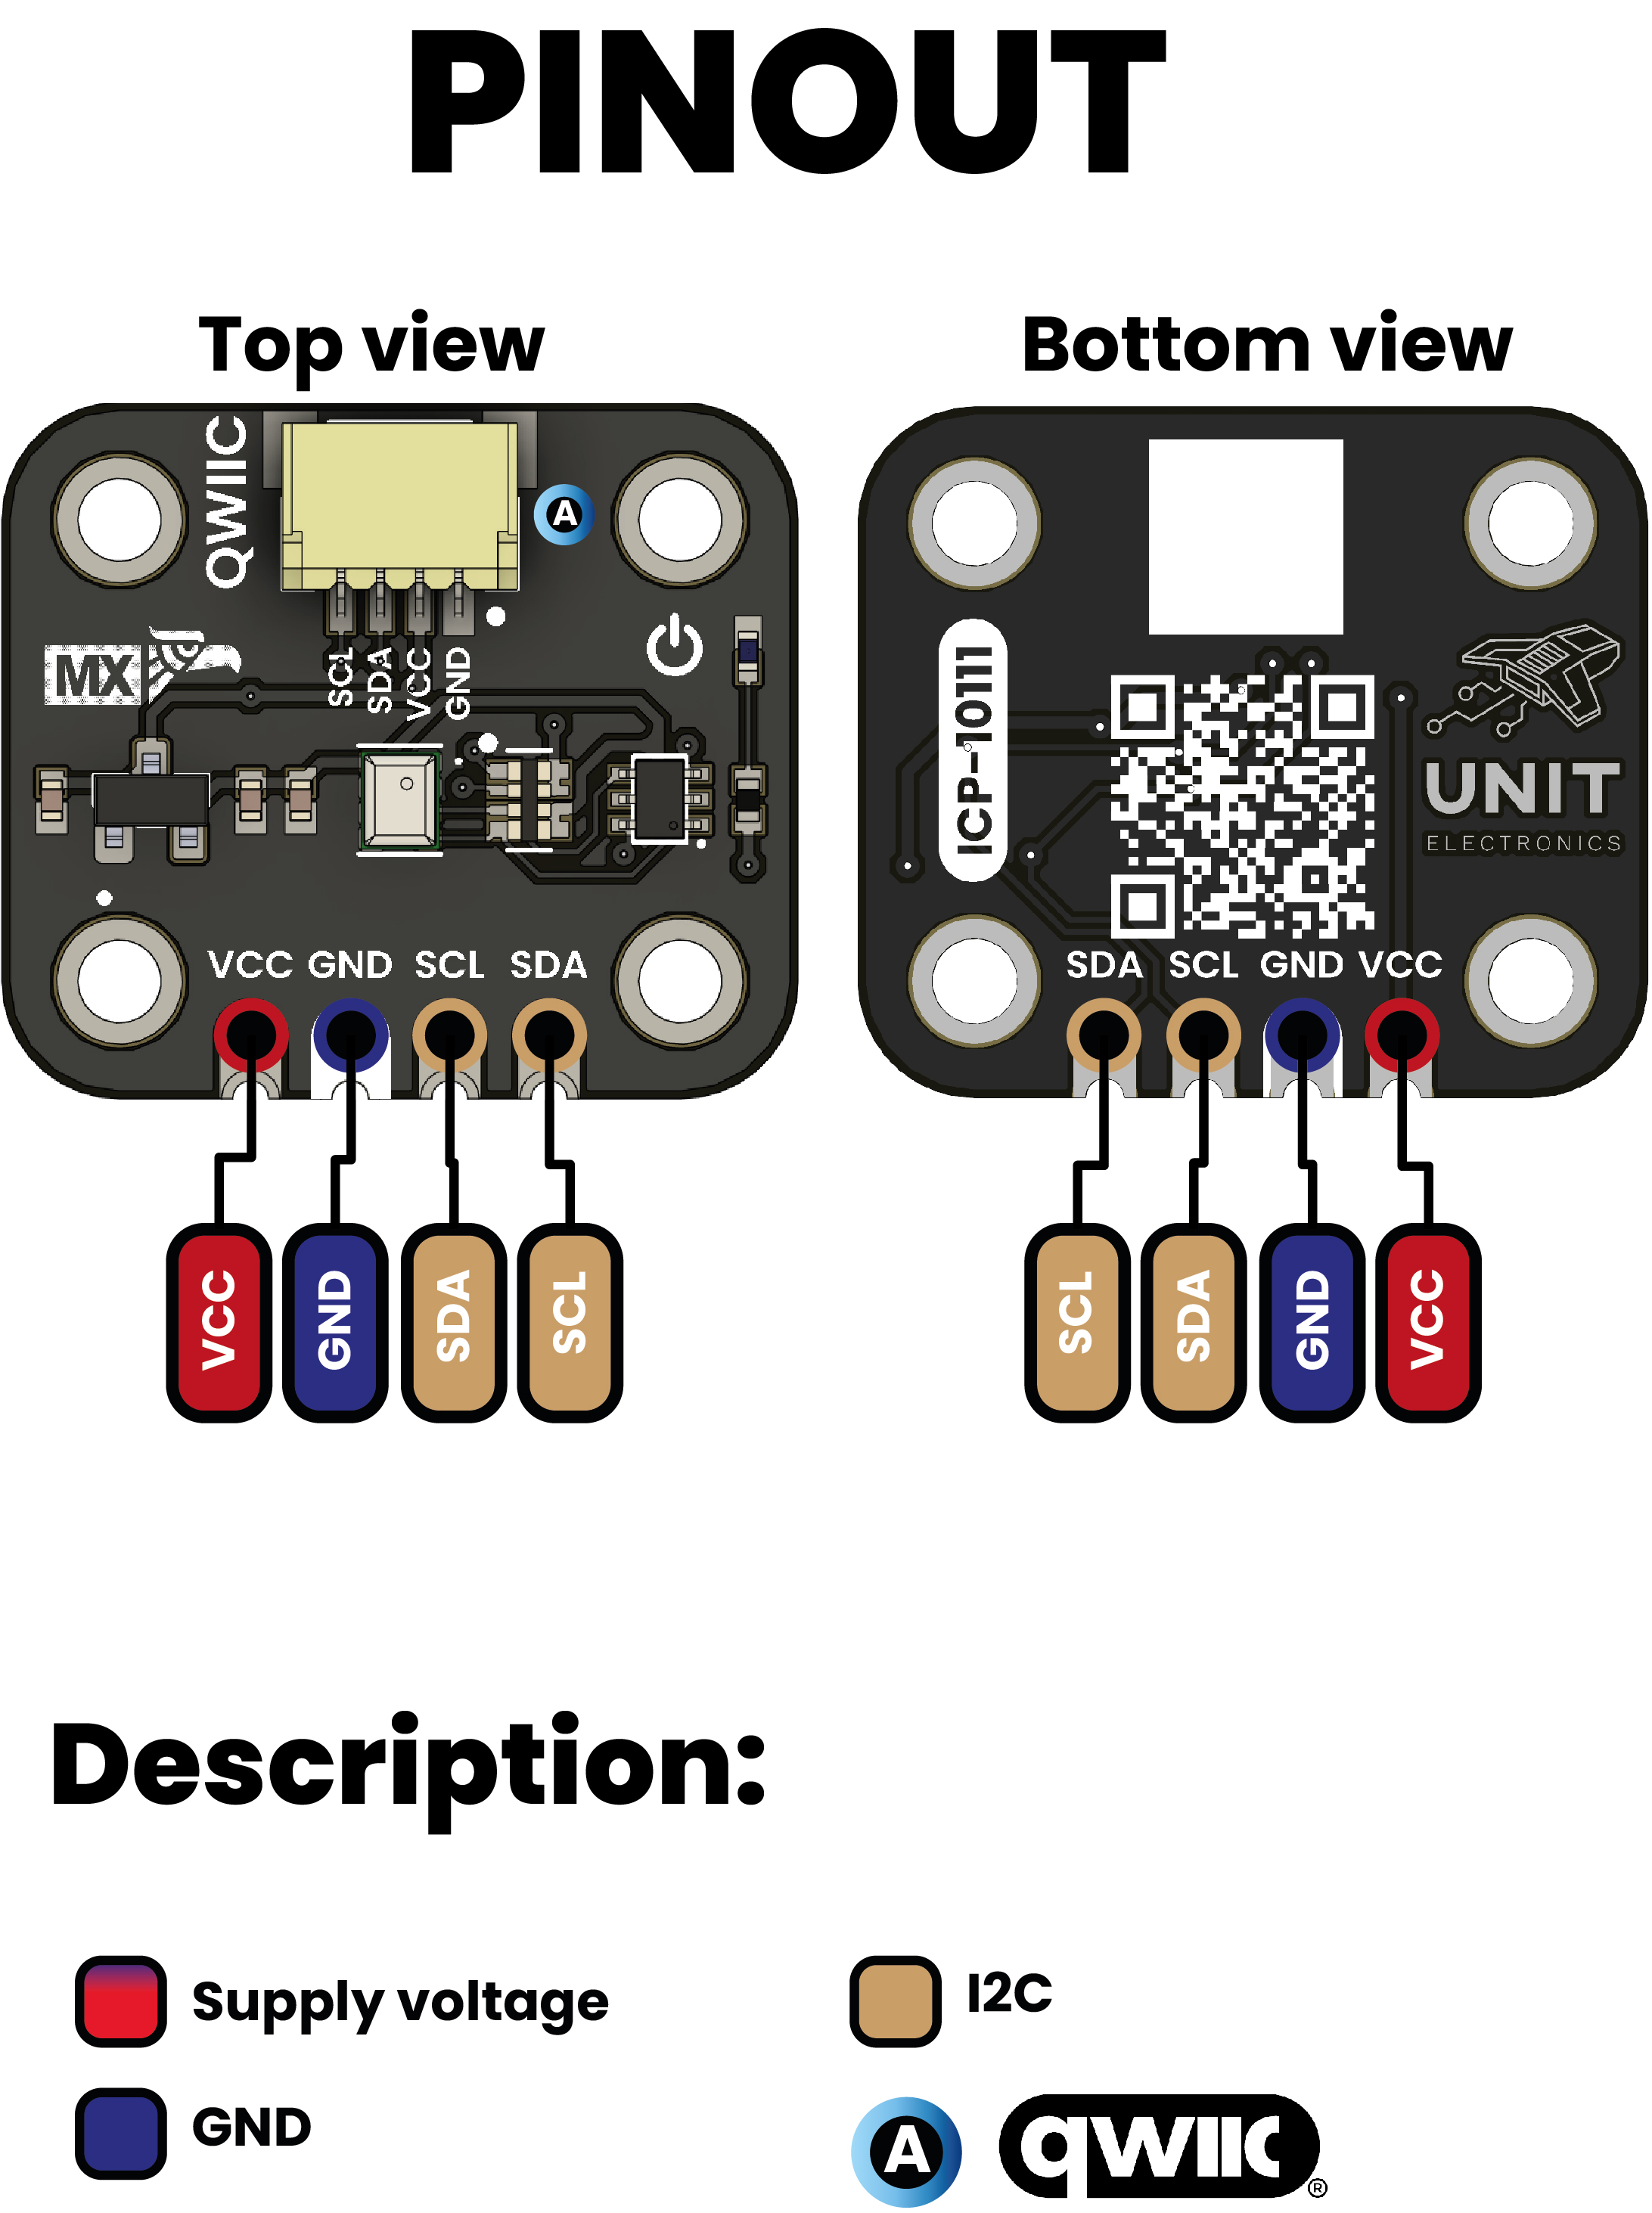
\includegraphics[width=0.9\textwidth]{es_unit_pinout_v_0_0_1_ue0094_icp10111_barometric_pressure_sensor_en.jpg}
\caption{Diagrama de Pines}
\label{fig:es-unit-pinout-v-0-0-1-ue0094-icp10111-barometric-pressure-sensor-en-jpg}
\end{figure}




\begin{table}[H]
\centering
\small
\begin{tabular}{|c|c|c|}
\hline
Etiqueta & Función & Notas \\
\hline
VCC & Alimentación & 3.3V o 5V \\
GND & Tierra & Tierra común para todos los componentes \\
SDA & Datos I2C & Línea de datos serie \\
SCL & Reloj I2C & Línea de reloj serie \\
\hline
\end{tabular}
\caption{Configuración de Pines}
\end{table}


\subsection{Dimensiones}


\begin{figure}[H]
\centering
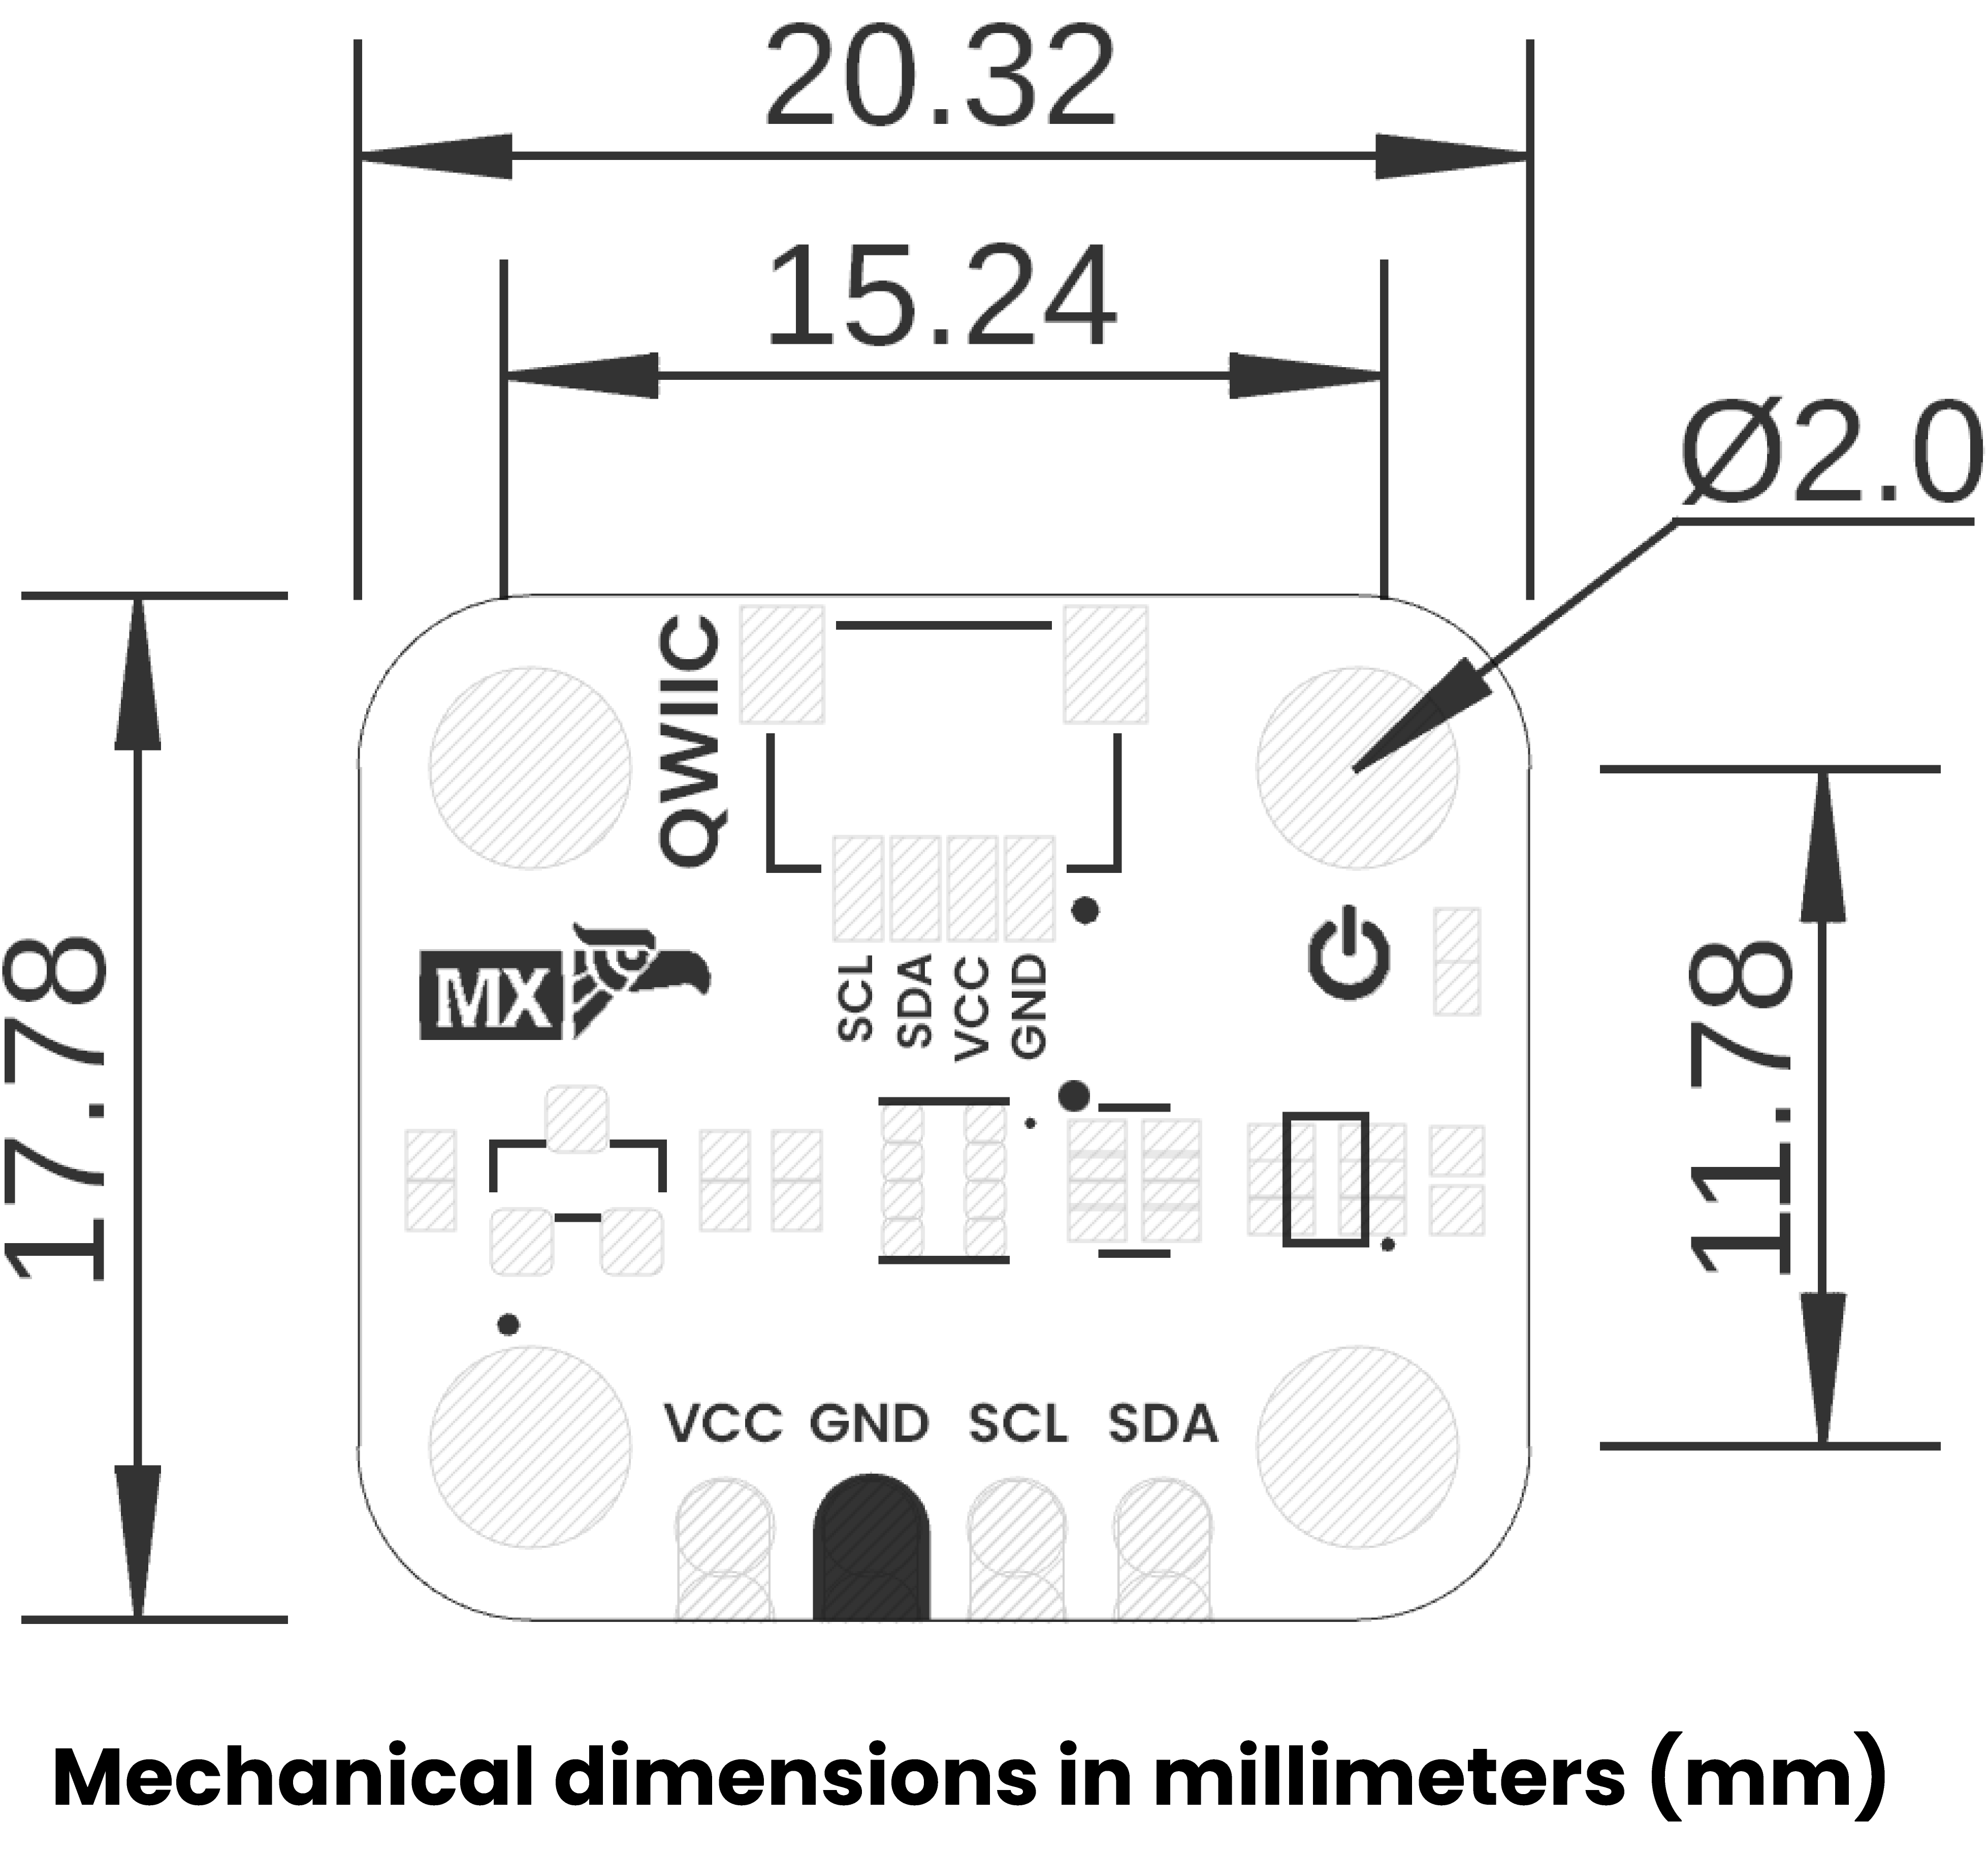
\includegraphics[width=0.6\textwidth]{es_unit_dimension_v_1_0_0_icp10111_barometric_pressure_sensor.png}
\caption{Dimensiones}
\label{fig:es-unit-dimension-v-1-0-0-icp10111-barometric-pressure-sensor-png}
\end{figure}



\subsection{Topología}


\begin{figure}[H]
\centering
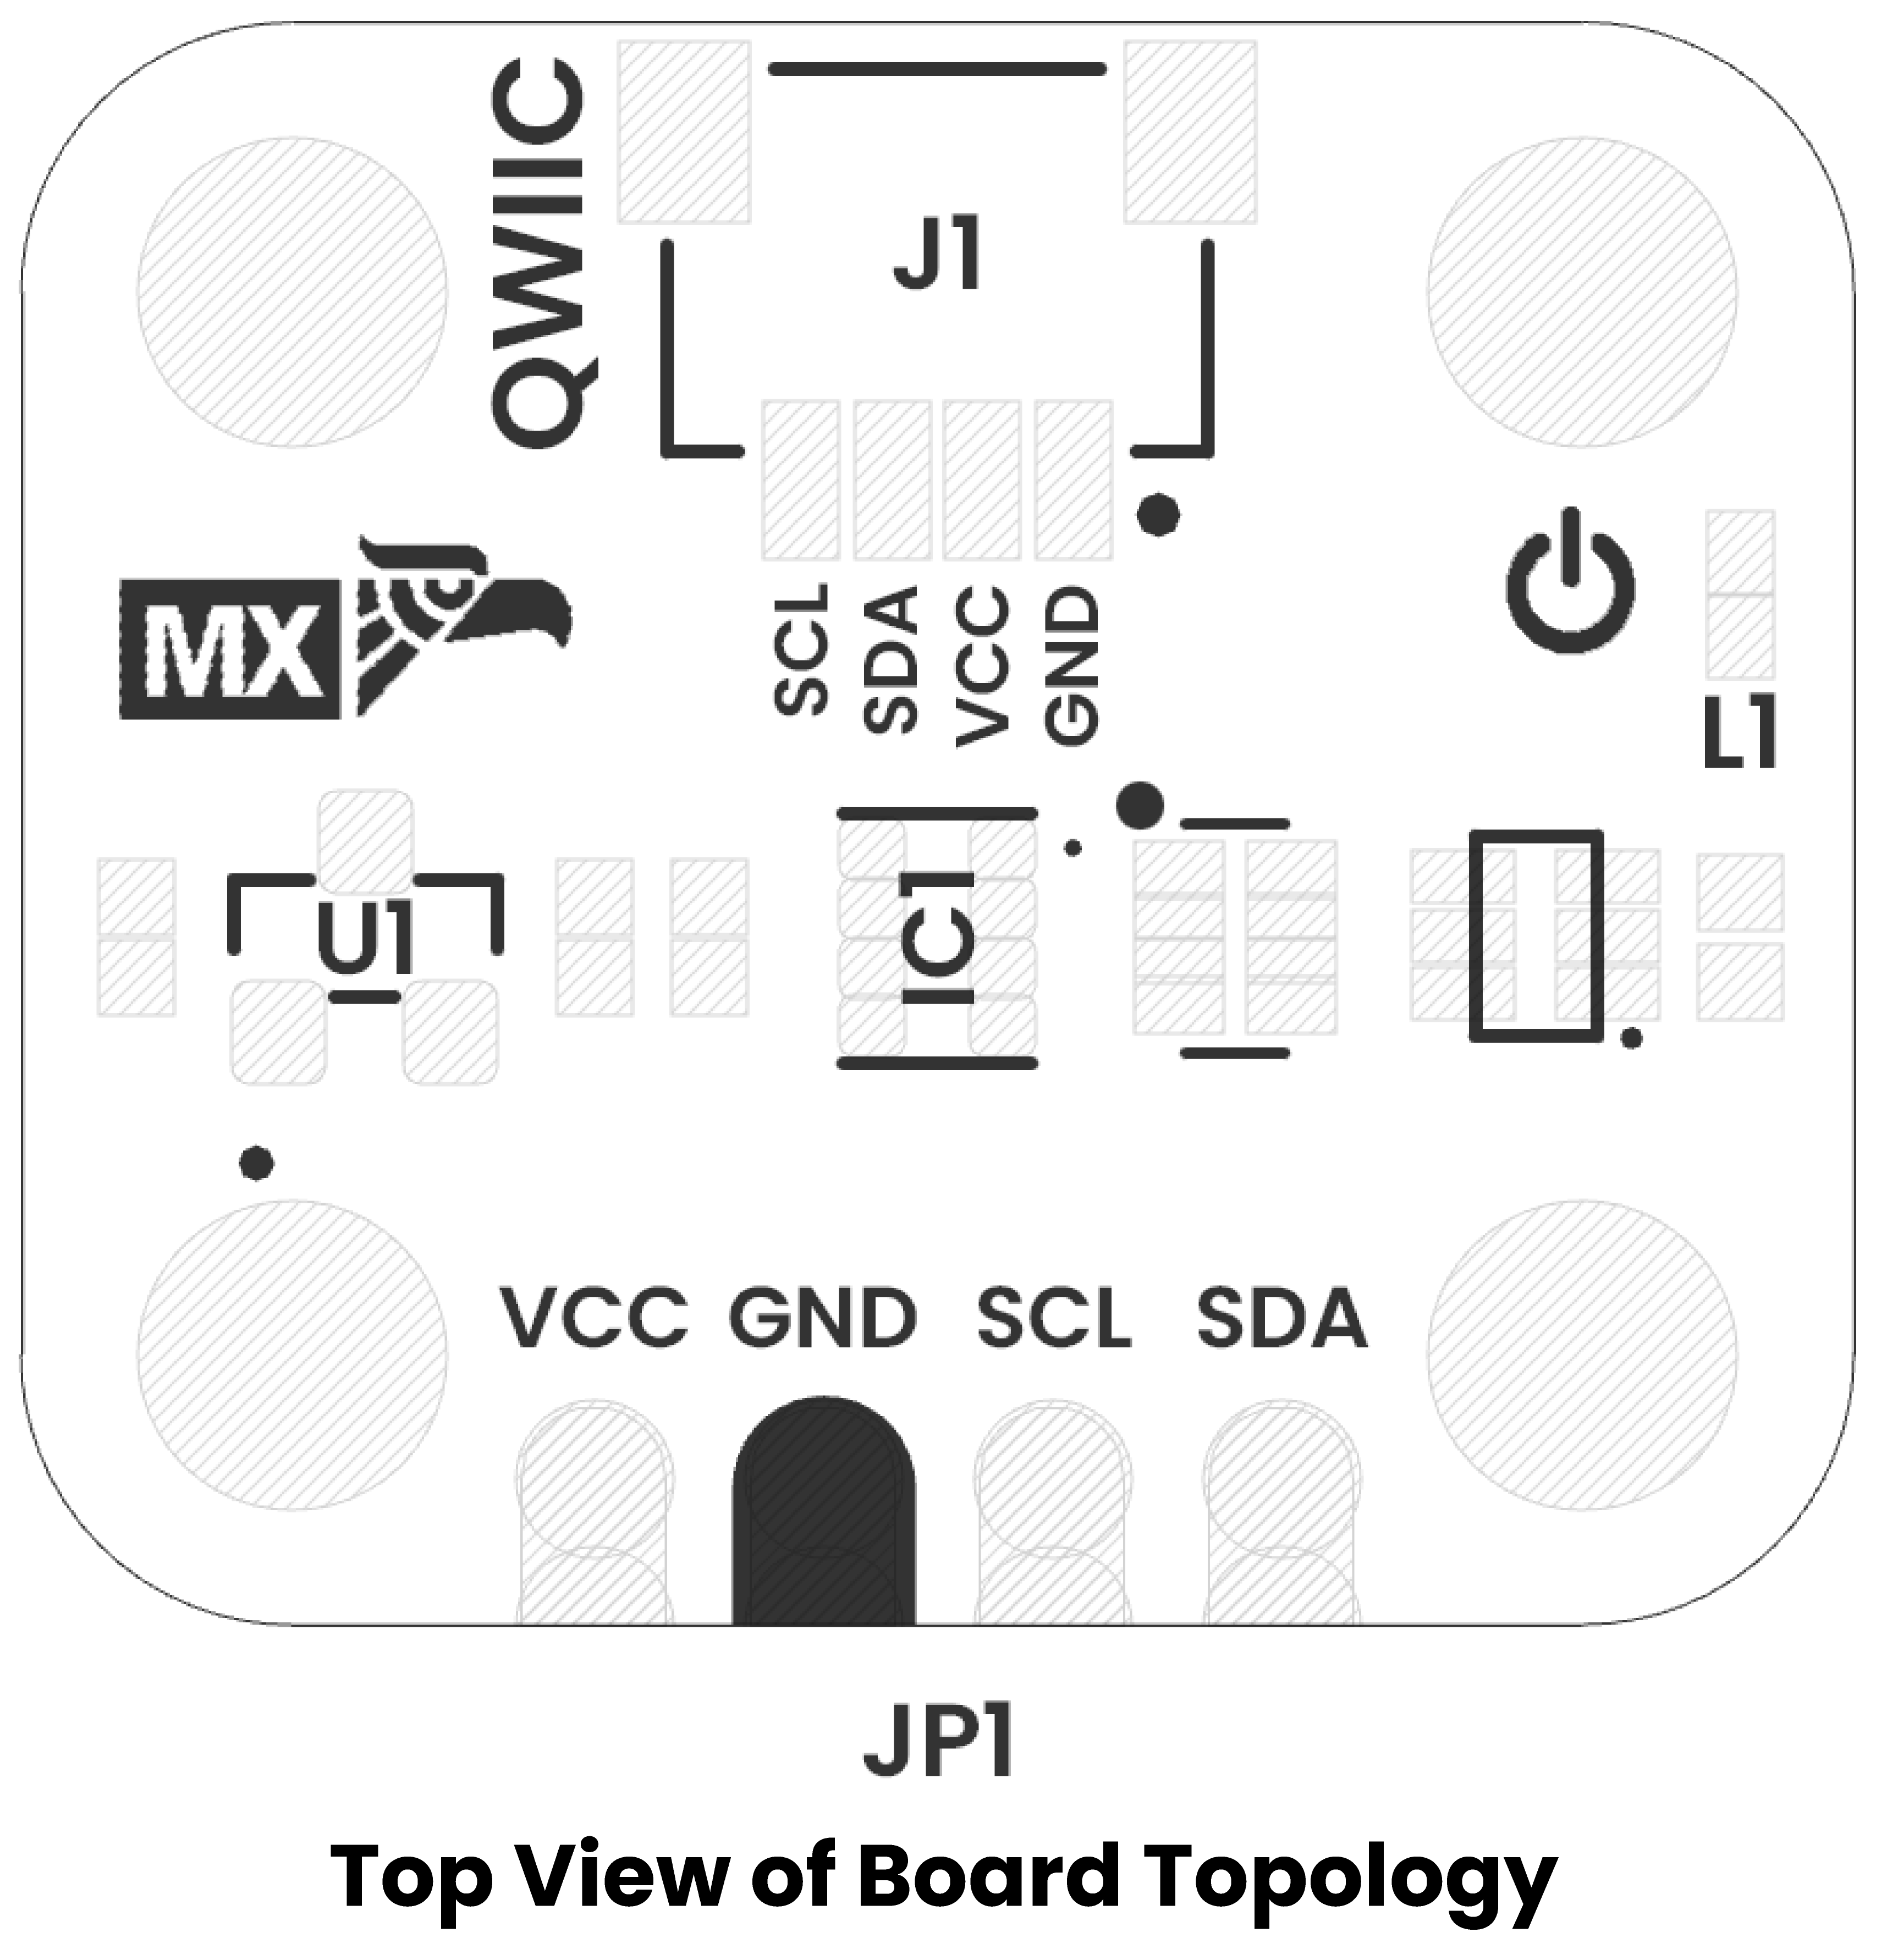
\includegraphics[width=0.7\textwidth]{es_unit_topology_v_1_0_0_icp10111_barometric_pressure_sensor.png}
\caption{Topología}
\label{fig:es-unit-topology-v-1-0-0-icp10111-barometric-pressure-sensor-png}
\end{figure}




\begin{table}[H]
\centering
\small
\begin{tabular}{|c|c|}
\hline
Ref. & Descripción \\
\hline
IC1 & Sensor de Presión Barométrica ICP-10111 \\
IC2 & Sensor Ambiental BME688 \\
L1 & LED de Encendido \\
U1 & Regulador ME6206A18XG 1.8V \\
JP1 & Orificios Castellanos de 2.54 mm \\
J1 & Conector QWIIC (JST paso 1 mm) para I2C \\
\hline
\end{tabular}
\caption{Referencia de Componentes}
\end{table}


\subsection{Interfaces de Comunicación}

\subsubsection{Interfaz I2C}
\begin{itemize}
\item \textbf{Dirección}: 0x63 (ICP-10111), 0x77 (BME688)
\item \textbf{Velocidad}: Estándar (100 kHz), Rápido (400 kHz)
\item \textbf{Características}: Conector compatible QWIIC
\item \textbf{Resistencias Pull-up}: 4.7k$\Omega$ integradas
\end{itemize}

\subsubsection{Especificaciones de Interfaz Digital}
\begin{itemize}
\item \textbf{Niveles Lógicos}: Compatible CMOS 3.3V
\item \textbf{Entrada Alta}: 2.0V mínimo
\item \textbf{Entrada Baja}: 0.8V máximo
\item \textbf{Corriente de Salida}: 4mA típico
\end{itemize}

\subsection{Características Físicas}

\subsubsection{Información del Encapsulado}


\begin{table}[H]
\centering
\small
\begin{tabular}{|c|c|c|}
\hline
Parámetro & Valor & Unidad \\
\hline
Tipo de Encapsulado & PCB Personalizado & - \\
Dimensiones & 25.4 x 15.24 x 3.2 & mm \\
Montaje & Orificios castellanos & Paso 2.54mm \\
Peso & 2.1 & g \\
\hline
\end{tabular}
\caption{Technical Specifications}
\end{table}


\subsubsection{Especificaciones Ambientales}


\begin{table}[H]
\centering
\small
\begin{tabular}{|l|l|l|l|l|}
\hline
Parámetro & Mín & Máx & Unidad & Condiciones \\
\hline
Temperatura de Operación & -40 & +85 & \degreeC & Precisión completa \\
Temperatura de Almacenamiento & -55 & +125 & \degreeC & - \\
Humedad & 0 & 100 & %HR & Sin condensación \\
Rango de Presión & 300 & 1250 & hPa & Presión absoluta \\
\hline
\end{tabular}
\caption{Technical Specifications}
\end{table}


\subsection{Soporte de Software}

\subsubsection{Entorno de Desarrollo}
\begin{itemize}
\item \textbf{Arduino IDE}: Soporte completo de librería
\item \textbf{ESP-IDF}: Integración de driver nativo
\item \textbf{PlatformIO}: Soporte multiplataforma
\item \textbf{CircuitPython}: Librería Python disponible
\end{itemize}

\subsubsection{Librerías Principales}
\begin{itemize}
\item Driver del sensor de presión ICP-10111
\item Librería del sensor ambiental BME688
\item Protocolos de comunicación I2C
\item Filtrado y calibración de datos
\end{itemize}

\subsection{Aplicaciones}

El módulo ICP-10111 es ideal para:

\begin{enumerate}
\item \textbf{Monitoreo Meteorológico}
\end{enumerate}
\begin{itemize}
\item Medición de presión atmosférica
\item Determinación de altitud
\item Sistemas de predicción meteorológica
\end{itemize}

\begin{enumerate}
\item \textbf{Sensores Ambientales IoT}
\end{enumerate}
\begin{itemize}
\item Automatización de edificios inteligentes
\item Monitoreo agrícola
\item Evaluación de calidad del aire
\end{itemize}

\begin{enumerate}
\item \textbf{Dispositivos Portátiles}
\end{enumerate}
\begin{itemize}
\item Rastreadores de fitness
\item Dispositivos de navegación al aire libre
\item Control de altitud de drones
\end{itemize}

\subsection{Seguridad y Cumplimiento}

\subsubsection{Certificaciones}
\begin{itemize}
\item \textbf{RoHS}: Cumple con directiva de la UE
\item \textbf{REACH}: Cumple con regulación de la UE
\item \textbf{CE}: Compatibilidad electromagnética
\end{itemize}

\subsubsection{Características de Seguridad}
\begin{itemize}
\item \textbf{Protección ESD}: $\pm$2kV HBM en todos los pines
\item \textbf{Protección de Polaridad Inversa}: Integrada
\item \textbf{Protección Térmica}: Monitoreo de rango de operación
\end{itemize}

\subsection{Referencias}

\begin{itemize}
\item \href{https://product.tdk.com/system/files/dam/doc/product/sensor/pressure/capacitive-pressure/data_sheet/ds-000177-icp-10111-v1.3.pdf}{Hoja de Datos ICP-10111}
\item \href{https://www.bosch-sensortec.com/media/boschsensortec/downloads/datasheets/bst-bme688-ds000.pdf}{Hoja de Datos BME688}
\item \href{https://www.microne.com.cn/uploads/file/20200904/ME6206.pdf}{Hoja de Datos Regulador ME6206}
\end{itemize}

\subsection{Información de Pedidos}


\begin{table}[H]
\centering
\small
\begin{tabular}{|l|l|l|l|}
\hline
Número de Parte & Descripción & Empaque & MOQ \\
\hline
ICP10111-001 & Módulo Estándar & Individual & 1 \\
ICP10111-DEV & Kit de Desarrollo & Caja de Kit & 1 \\
ICP10111-BULK & Pedido en Lote & Bandeja & 100 \\
\hline
\end{tabular}
\caption{Technical Specifications}
\end{table}


\subsection{Esquemáticos}


\begin{figure}[H]
\centering

\includegraphics[width=\textwidth]{es_Schematics_icon.jpg}
\caption{Esquemático del Circuito}
\label{fig:es-Schematics-icon-jpg}
\end{figure}



---

\textit{Para soporte técnico e información adicional, visita nuestro sitio web o contacta a nuestro equipo de ingeniería.}


\end{document}
